%!TEX root=../oi-magistr-si.tex
\section[OSP - Přenositelnost, multiplatformnost]{Požadavky a pravidla pro tvorbu přenositelného kódu. Organizace projektů a struktura operačních systémů pro zajištění přenositelnosti mezi různými platformami (OS, CPU). Vnitřní a vnější reprezentace dat, převody mezi nimi, vztah k síťovým protokolům (endianing, serializace atd.)}

\subsection{Požadavky a pravidla pro tvorbu přenositelného kódu}
Při realizaci softwarových systémů často nemůžeme zanedbat cílovou hardwarovou architekturu stroje a musíme psát kód tak, aby jej bylo možné snadno upravit (ideálně pouze rekompilovat) pro běh na jiných platformách. V okamžiku kdy je nutné přímo interagovat s některou hardwarovou komponentou počítače (řídící jednotky, SCADA systémy, $\hdots$), se dostáváme až na úroveň, kdy musíme řešit věci, jako uspořádání bytů v proměnné apod. K základním požadavkům na přenositelnost zdrojového kódu patří:

\begin{itemize}[itemsep=0px]
\item psát čistě a používat jen to, co je jazykem deklarováno,
\item pokud je to možné používat pouze standardizovaná API - POSIX, IEEE Std. 1003.1,
\item nepředpokládat pořadí byte/char ve slovech - little versus big endian,
\item nepředpokládat počet bitů v adresační jednotce (používat stdint.h - int32\_t, $\hdots$),
\item psát kód proti knihovnám a nikoliv přímo proti konkrétním voláním služeb operačního systému (konkrétním makrům, číslům volání, atd.).
\end{itemize}

\subsection{Organizace projektů a struktura operačních systémů pro zajištění přenositelnosti mezi různými platformami (OS, CPU)}

Aby bylo možné snadno přenášet projekty mezi různými operačními systémy a jejich verzemi a hardwarovými architekturami, bylo definováno několik standardů a vyvinuto několik nástrojů, které mají tuto přenositelnost usnadnit:
\paragraph{POSIX} - Portable Operating System Interface - standardy IEEE 1003 a ISO/IEC 9945 - definuje, co by měl poskytovat operační systém, jaké příkazy, jaké vlastnosti - na základě tohoto standardu je potom poměrně snadné převádět projekty mezi různými distribucemi Linuxu, UNIXY, atd. (uvádí se, že to je mnohdy jednodušší než převod projektů mezi různými verzemi Windows).

\paragraph{Filesystem hierarchy standard (FHS)} - dokument popisující, co má být ve kterém adresáři v linuxové distribuci, mezi typické adresáře patří
\begin{itemize}[itemsep=0px]
\item \texttt{/usr/bin} - binární programy (platformně závislé)
\item \texttt{/usr/local} - prefix do kterého je instalován software lokální pro tento stroj
\item \texttt{/usr/share} - sdílené (na hw platformě nezávislé) zdroje - často může být tento systém sdílen mezi různými stroji (např. pomocí NFS)
\item \texttt{/usr/lib} - knihovny (platformně závislé)
\item FHS popisuje, co by měl/neměl který adresář správně obsahovat
\end{itemize}

\subsection{Kompilace GNU balíků}
Nejrozšířenějším nástrojem pro kompilaci GNU balíků je systém Autotools. Tento systém se skládá z více nástrojů. Mezi hlavní a nejdůležitější patří:
\begin{itemize}[itemsep=0px]
\item m4, aclocal, autoheader
\item autoheader
\item autoconf
\item automake
\end{itemize}

Tyto nástroje zpracovávají vstupní soubory, které obsahují informace o projektu, závislostech, požadavcích na cílovou platformu atd. Jedná se zejména o soubory: \texttt{Makefile.am}, \texttt{configure.ac}, \texttt{config.h.in}.

Proces sestavování (build) softwarového balíku se dělí na část, která probíhá u vývojáře (vyžaduje ke svému běhu větší množinu nástrojů) a část, kterou spouští klient.

\subsection{Portace kódu a křížový překlad}
Většinou není nutné, aby každý uživatel kompiloval software ze zdrojových kódů. Je možné dodávat konkrétní verzi zkompilovanou pro cílovou platformu. Pro sestavení programu se používá build toolchain (v případě použití GCC se označuje jako GNU Tool Chain). Ten zahrnuje jednak vlastní kompiler (např. GCC - GNU Compiler Collection) a dále nástroje pro vytváření knihoven, linker atd.

Tento toolchain může kompilovat kód pro různé platformy. Na základě toho rozeznáváme native toolchain a cross-compiling toolchain (výsledné binární soubory běží na platformě toolchainu nebo na jiné platformě).

\begin{figure}[h!]
\centering
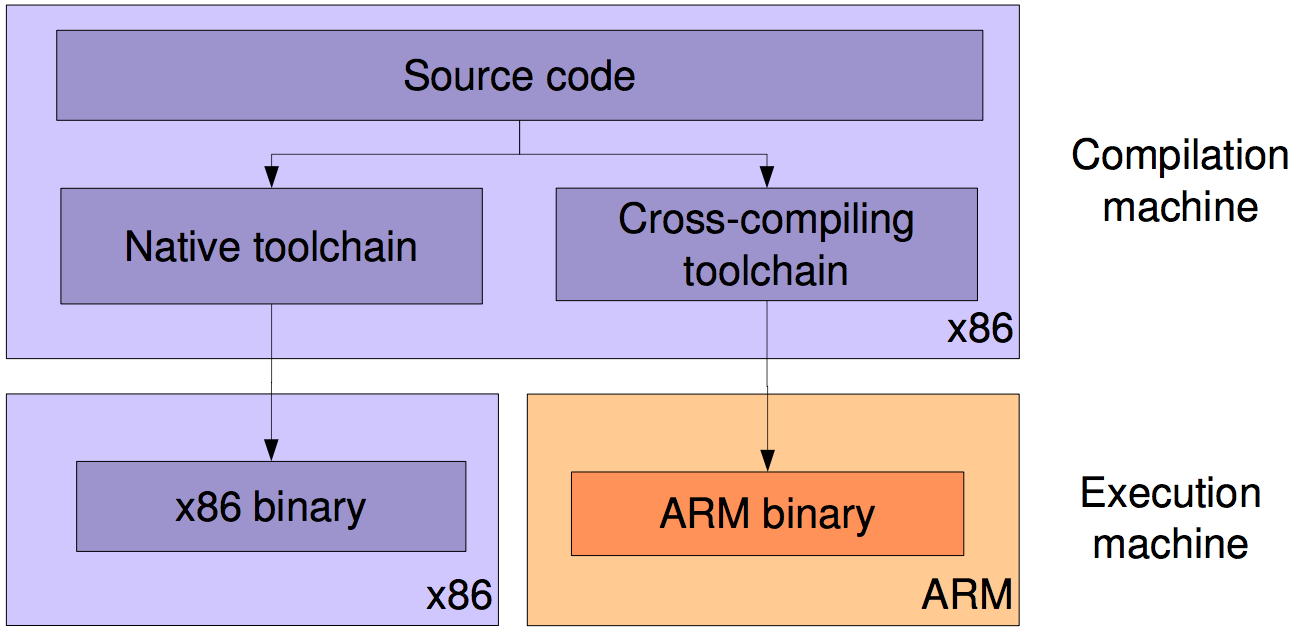
\includegraphics[width=130mm]{08/images/portace-kodu}
\end{figure}

\subsection{Konverze vnitřních a vnějších/síťových formátů dat}

Na to je tam slajd.. endianita, rozsah cisel
https://rtime.felk.cvut.cz/osp/prednasky/osp-hw-and-porting.pdf

\begin{itemize}[itemsep=0px]
\item little endian/big endian
\item textové formáty: XML, HTML, SOAP, JSON
\item XDR (external data representation) - nezávislý na arch. systému, od roku 1995 IETF standard
\item RPC, CORBA
\item padding - zarovnávání packetů
\end{itemize}